\begin{enumerate}[label=\thesubsection.\arabic*, ref=\thesubsection.\theenumi]
\item
If tangents $PA$ and $PB$ drawn from an external point $P$ to a circle with centre $O$ are inclined to each other at an angle of $80^\circ$, then $\angle POA$ is equal to
\hfill (CBSE 2025 Set 2, Q.1)
\begin{enumerate}
	\begin{multicols}{4}
    \item $40^\circ$
    \item $50^\circ$
    \item $60^\circ$
    \item $80^\circ$
	\end{multicols}
\end{enumerate}
\begin{figure}[H]
	\centering
\begin{tikzpicture}[scale=1.1, >=Stealth]
    \coordinate (O) at (0,0);
    \coordinate (P) at (-3.1114,0);
    \coordinate (A) at (-1.2856,1.5321);
    \coordinate (B) at (-1.2856,-1.5321);
    \draw[thick] (O) circle (2);
    \draw[thick] (P) -- (A) -- (O) -- (B) -- (P);
    \draw[thick] (P) -- (O);
    \fill (O) circle (1.5pt) (P) circle (1.5pt) (A) circle (1.5pt) (B) circle (1.5pt);
    % right-angle marks at the points of contact
    \draw (-1.1570,1.3789) -- (-1.3102,1.2503) -- (-1.4388,1.4035);
    \draw (-1.1570,-1.3789) -- (-1.3102,-1.2503) -- (-1.4388,-1.4035);
    \node[right] at (O) {$O$};
    \node[left] at (P) {$P$};
    \node[above left] at (A) {$A$};
    \node[below left] at (B) {$B$};
    \draw (P)++(0.7,0) arc[start angle=0, end angle=40, radius=0.7];
    \draw (P)++(0.7,0) arc[start angle=0, end angle=-40, radius=0.7];
    \node[fill=white, inner sep=1pt] at (-2.15,0.0) {\small $80^\circ$};
\end{tikzpicture}

	\caption{Tangents $PA$ and $PB$}
	\label{fig:CBSE25S2-q1}
\end{figure}

\solution
A radius is perpendicular to the tangent at the point of contact. Hence,
\begin{align}
	\angle OAP = \angle OBP = 90^\circ
\end{align}
In the quadrilateral $AOBP$,
\begin{align}
	\angle AOB + \angle OAP + \angle APB + \angle OBP &= 360^\circ
	\\
	\implies \angle AOB &= 360^\circ - 90^\circ - 80^\circ - 90^\circ = 100^\circ
\end{align}
Since $OA = OB$ (radii), $PA = PB$ (tangents from an external point) and $OP$ is common, $\triangle OAP \cong \triangle OBP$, so $OP$ bisects $\angle AOB$. Therefore,
\begin{align}
	\angle POA = \frac{\angle AOB}{2} = 50^\circ \quad \brak{\text{Option B}}
\end{align}
The following code verifies the solution
\begin{lstlisting}[frame=single, basicstyle=\rmfamily, escapeinside={(*@}{@*)}]
(*@\makebox[\dimexpr\linewidth-2\fboxsep-2\fboxrule\relax][c]{codes/1.c}@*)
\end{lstlisting}

\item
The volumes of two cubes are in the ratio $8:125$. The ratio of their surface areas is
\hfill (CBSE 2025 Set 2, Q.3)
\begin{enumerate}
    \begin{multicols}{4}
        \item $8:125$
        \item $4:25$
        \item $2:5$
        \item $16:25$
    \end{multicols}
\end{enumerate}


\solution
Let the sides of the cubes be $a$ and $b$. Then
\begin{align}
	\frac{a^3}{b^3} = \frac{8}{125} \implies \frac{a}{b} = \sqrt[3]{\frac{8}{125}} = \frac{2}{5}
\end{align}
The surface area of a cube of side $a$ is $6a^2$. Hence,
\begin{align}
	\frac{S_1}{S_2} = \frac{6a^2}{6b^2} = \brak{\frac{a}{b}}^2 = \frac{4}{25}
	\implies S_1 : S_2 = 4 : 25 \quad \brak{\text{Option B}}
\end{align}
The following code verifies the solution
\begin{lstlisting}[frame=single, basicstyle=\rmfamily, escapeinside={(*@}{@*)}]
(*@\makebox[\dimexpr\linewidth-2\fboxsep-2\fboxrule\relax][c]{codes/3.c}@*)
\end{lstlisting}

\item
Two vertices of $\triangle PQR$ are $P\brak{-1,5}$ and $Q\brak{5,2}$. The coordinates of the point $R$ on $PQ$ which divides $PQ$ in the ratio $2:1$ are
\hfill (CBSE 2025 Set 2, Q.4)
\begin{enumerate}
	\begin{multicols}{4}
    \item $\brak{3,-3}$
    \item $\brak{5,5}$
    \item $\brak{3,3}$
    \item $\brak{5,1}$
	\end{multicols}
\end{enumerate}

\solution
Let $\vec{P} = \myvec{-1 \\ 5}$ and $\vec{Q} = \myvec{5 \\ 2}$. The displacement from $P$ to $Q$ is
\begin{align}
	\vec{Q} - \vec{P} = \myvec{6 \\ -3}
\end{align}
Since $PR : RQ = 2:1$, the point $R$ lies two-thirds of the way from $P$ to $Q$:
\begin{align}
	\vec{R} = \vec{P} + \frac{2}{3}\brak{\vec{Q}-\vec{P}} = \myvec{-1 \\ 5} + \myvec{4 \\ -2} = \myvec{3 \\ 3} \quad \brak{\text{Option C}}
\end{align}
The following code verifies the solution
\begin{lstlisting}[frame=single, basicstyle=\rmfamily, escapeinside={(*@}{@*)}]
(*@\makebox[\dimexpr\linewidth-2\fboxsep-2\fboxrule\relax][c]{codes/4.c}@*)
\end{lstlisting}
The following code generates \figref{fig:CBSE25S2-q4}.
\begin{lstlisting}[frame=single, basicstyle=\rmfamily, escapeinside={(*@}{@*)}]
(*@\makebox[\dimexpr\linewidth-2\fboxsep-2\fboxrule\relax][c]{codes/4plot.py}@*)
\end{lstlisting}
\begin{figure}[H]
	\centering
	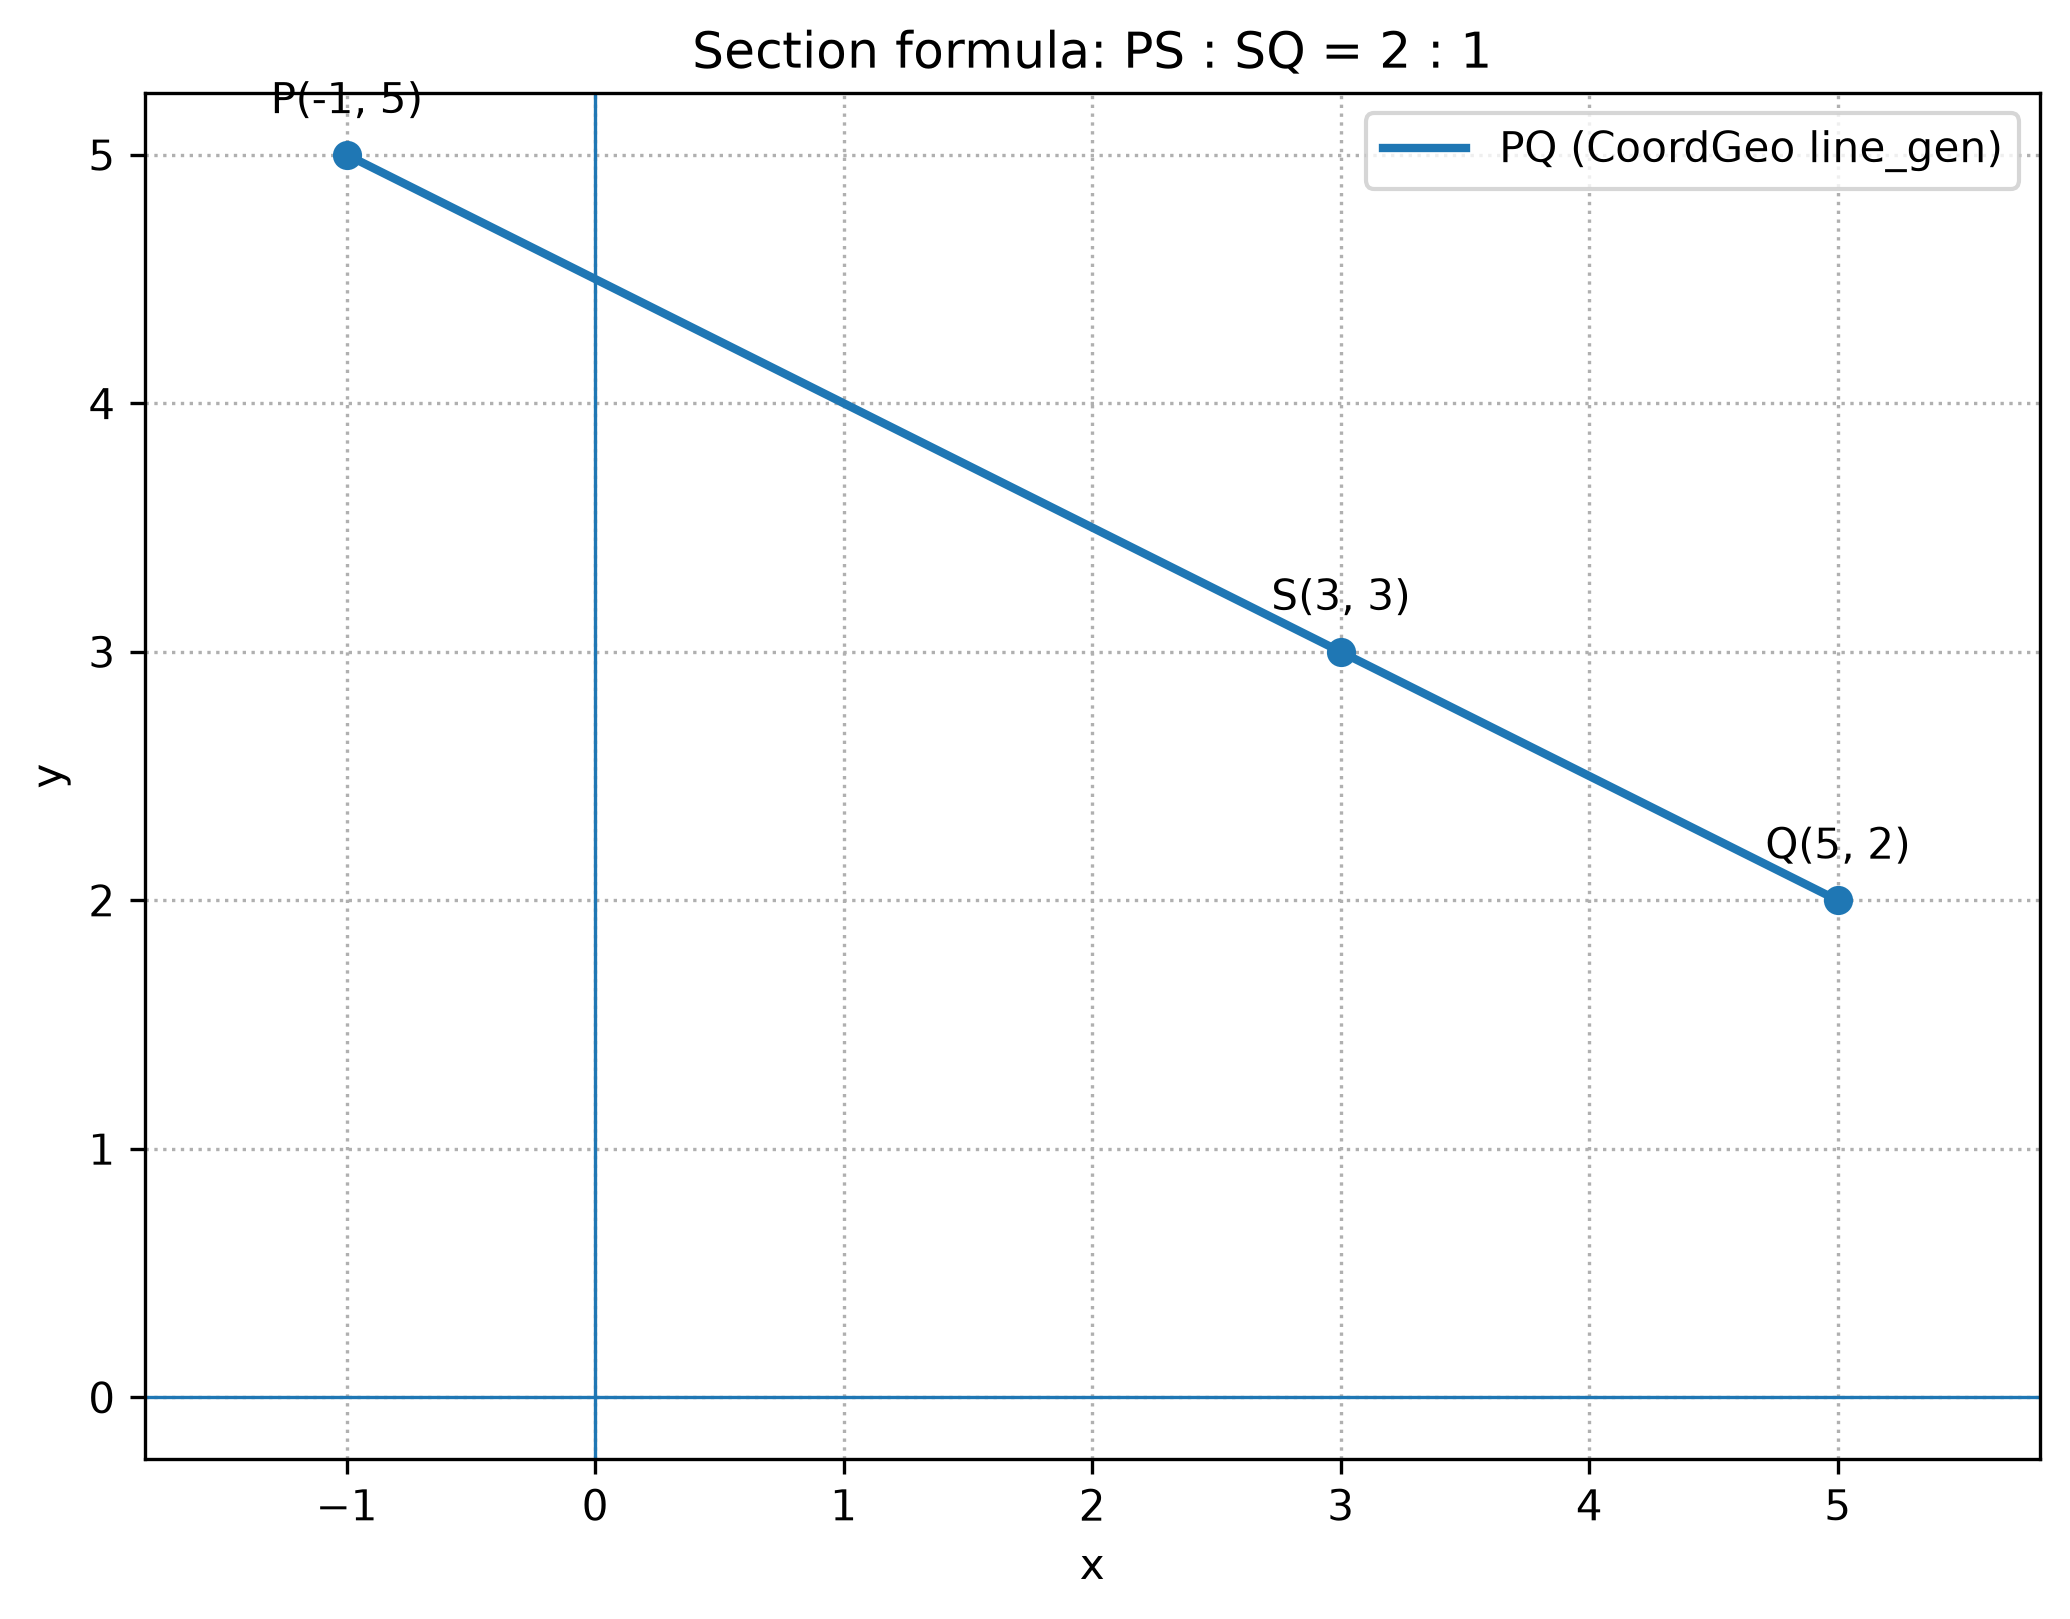
\includegraphics[width=0.5\linewidth]{figs/q4.png}
	\caption{Point $R$ dividing $PQ$ in the ratio $2:1$}
	\label{fig:CBSE25S2-q4}
\end{figure}

\item
If $\sin 4\theta = \frac{\sqrt{3}}{2}$, then $\frac{\theta}{3}$ is equal to
\hfill (CBSE 2025 Set 2, Q.5)
\begin{enumerate}
	\begin{multicols}{4}
    \item $60^\circ$
    \item $20^\circ$
    \item $15^\circ$
    \item $5^\circ$
	\end{multicols}
\end{enumerate}

\solution
Taking the principal (acute) value,
\begin{align}
	4\theta = \sin^{-1}\brak{\frac{\sqrt{3}}{2}} = 60^\circ
	\implies \theta = 15^\circ
	\implies \frac{\theta}{3} = 5^\circ \quad \brak{\text{Option D}}
\end{align}
The following code verifies the solution
\begin{lstlisting}[frame=single, basicstyle=\rmfamily, escapeinside={(*@}{@*)}]
(*@\makebox[\dimexpr\linewidth-2\fboxsep-2\fboxrule\relax][c]{codes/5.c}@*)
\end{lstlisting}

\item
The zeroes of the polynomial $p\brak{y} = 7y^2 - \frac{11}{3}y - \frac{2}{3}$ are
\hfill (CBSE 2025 Set 2, Q.6)
\begin{enumerate}
    \begin{multicols}{4}
        \item $\displaystyle -\frac{2}{3},-\frac{1}{7}$
        \item $\displaystyle -\frac{2}{7},-\frac{1}{3}$
        \item $\displaystyle \frac{2}{3},\frac{1}{7}$
        \item $\displaystyle \frac{2}{3},-\frac{1}{7}$
    \end{multicols}
\end{enumerate}

\solution
Multiplying by $3$, the zeroes of $p$ are the zeroes of
\begin{align}
	g\brak{y} = 21y^2 - 11y - 2, \quad g^{\prime}\brak{y} = 42y - 11
\end{align}
The Newton--Raphson iteration is
\begin{align}
	y_{n+1} = y_n - \frac{g\brak{y_n}}{g^{\prime}\brak{y_n}} = y_n - \frac{21y_n^2 - 11y_n - 2}{42y_n - 11}
\end{align}
Starting from $y_0 = 0.7$ and $y_0 = -0.2$, the iterations converge to
\begin{align}
	y = \frac{2}{3}, \quad y = -\frac{1}{7} \quad \brak{\text{Option D}}
\end{align}
which agree with the factorisation $g\brak{y} = \brak{3y-2}\brak{7y+1}$. The following code verifies the solution
\begin{lstlisting}[frame=single, basicstyle=\rmfamily, escapeinside={(*@}{@*)}]
(*@\makebox[\dimexpr\linewidth-2\fboxsep-2\fboxrule\relax][c]{codes/6.c}@*)
\end{lstlisting}
The following code generates \figref{fig:CBSE25S2-q6}.
\begin{lstlisting}[frame=single, basicstyle=\rmfamily, escapeinside={(*@}{@*)}]
(*@\makebox[\dimexpr\linewidth-2\fboxsep-2\fboxrule\relax][c]{codes/6plot.py}@*)
\end{lstlisting}
\begin{figure}[H]
	\centering
	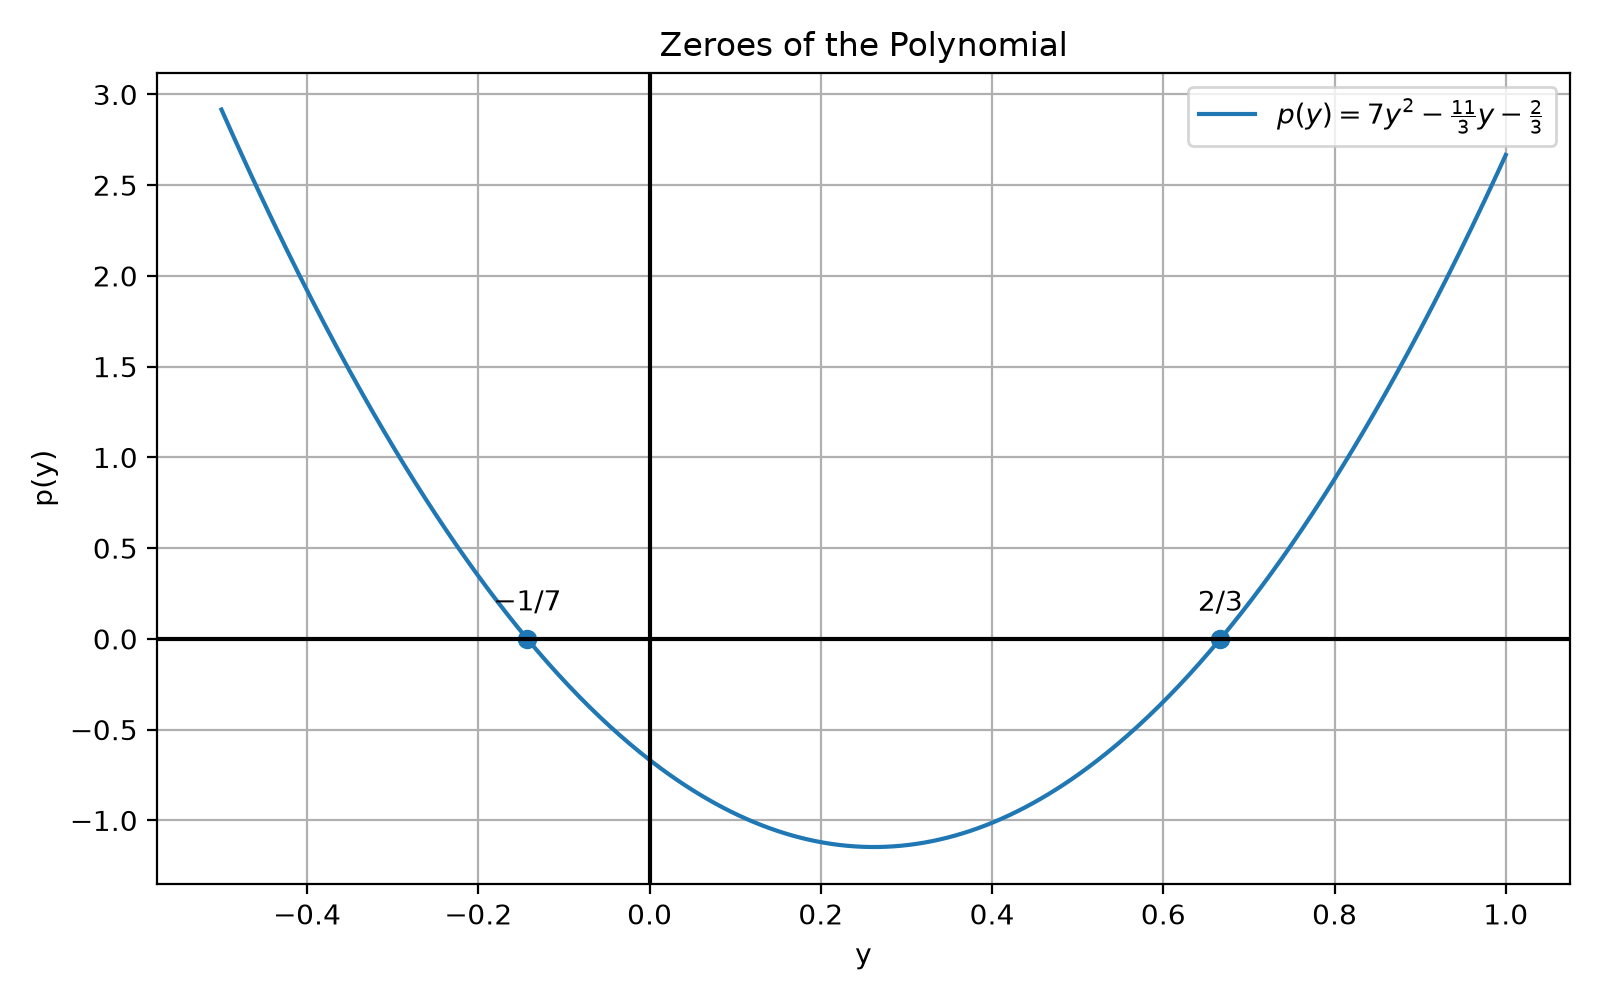
\includegraphics[width=0.6\linewidth]{figs/q6.png}
	\caption{Graph of $p\brak{y}$ and its zeroes}
	\label{fig:CBSE25S2-q6}
\end{figure}

\item
$AOBC$ is a rectangle whose three vertices are $A\brak{0,2}$, $O\brak{0,0}$ and $B\brak{4,0}$. The square of the length of its diagonal is
\hfill (CBSE 2025 Set 2, Q.8)
\begin{enumerate}
	\begin{multicols}{4}
    \item $36$
    \item $20$
    \item $16$
    \item $4$
	\end{multicols}
\end{enumerate}

\solution
The fourth vertex is $C\brak{4,2}$ and the diagonal is $AB$. With $\vec{A} = \myvec{0\\2}$, $\vec{B} = \myvec{4\\0}$,
\begin{align}
	\vec{B} - \vec{A} = \myvec{4 \\ -2}, \qquad
	\norm{\vec{B}-\vec{A}}^2 = \brak{\vec{B}-\vec{A}}^{\top}\brak{\vec{B}-\vec{A}} = 16 + 4 = 20 \quad \brak{\text{Option B}}
\end{align}
The following code verifies the solution
\begin{lstlisting}[frame=single, basicstyle=\rmfamily, escapeinside={(*@}{@*)}]
(*@\makebox[\dimexpr\linewidth-2\fboxsep-2\fboxrule\relax][c]{codes/8.c}@*)
\end{lstlisting}
The following code generates \figref{fig:CBSE25S2-q8}.
\begin{lstlisting}[frame=single, basicstyle=\rmfamily, escapeinside={(*@}{@*)}]
(*@\makebox[\dimexpr\linewidth-2\fboxsep-2\fboxrule\relax][c]{codes/8plot.py}@*)
\end{lstlisting}
\begin{figure}[H]
	\centering
	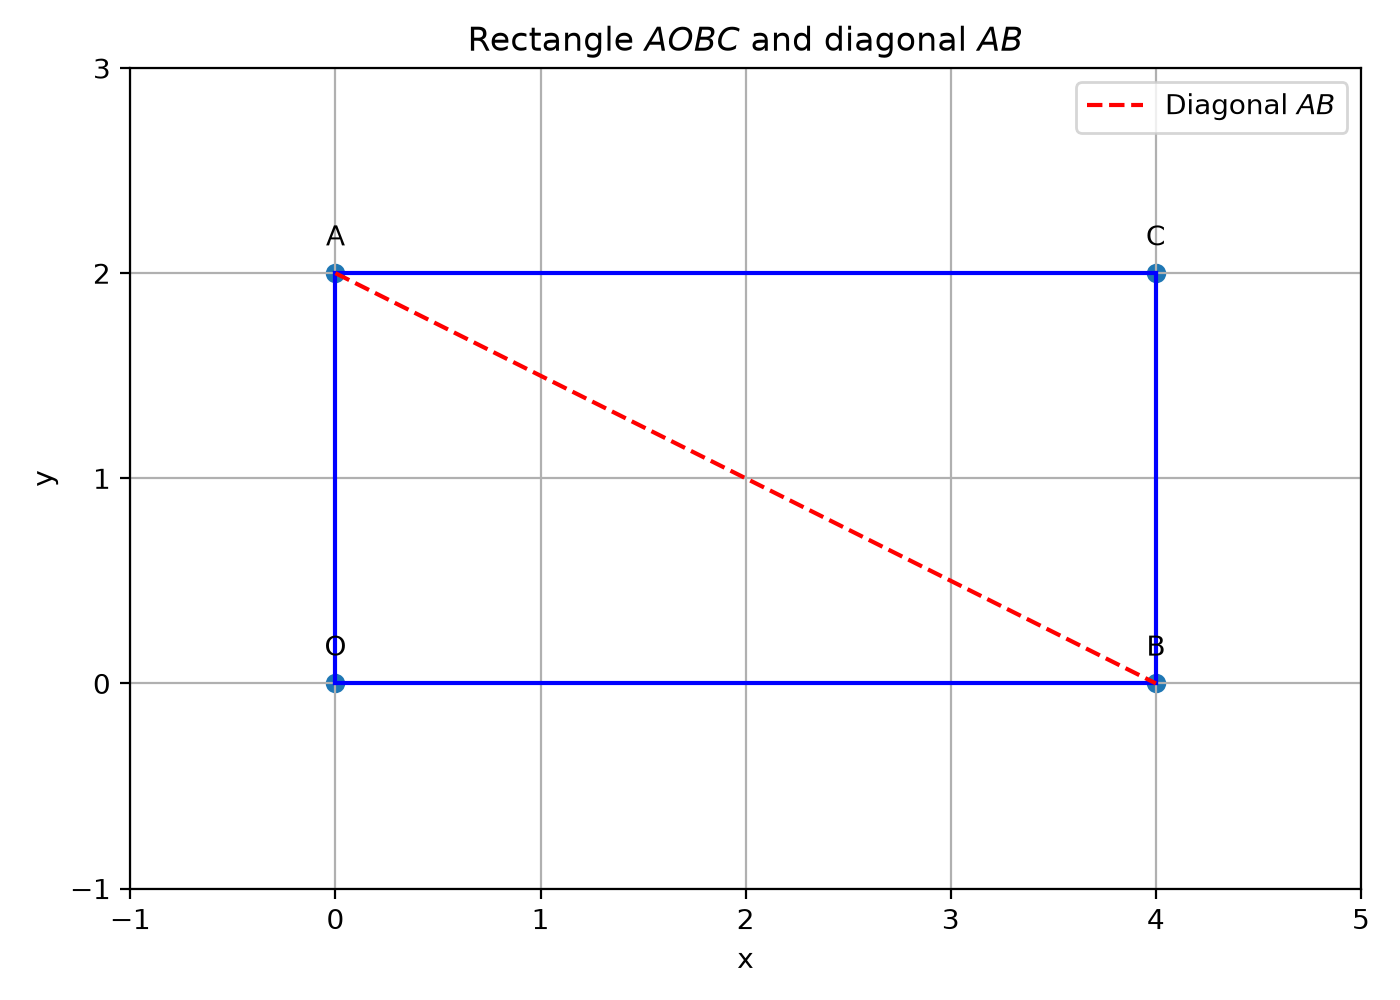
\includegraphics[width=0.55\linewidth]{figs/q8.png}
	\caption{Rectangle $AOBC$ and its diagonals}
	\label{fig:CBSE25S2-q8}
\end{figure}

\item
If $x$ is the LCM of $4, 6, 8$, $y$ is the LCM of $3, 5, 7$ and $p$ is the LCM of $x$ and $y$, then
\hfill (CBSE 2025 Set 2, Q.9)
\begin{enumerate}
	\begin{multicols}{4}
    \item $p = 35x$
    \item $p = 4y$
    \item $p = 8x$
    \item $p = 16y$
	\end{multicols}
\end{enumerate}

\solution
The Euclidean algorithm gives $\gcd\brak{a,b} = \gcd\brak{b, a \bmod b}$, and
\begin{align}
	\text{lcm}\brak{a,b} = \frac{ab}{\gcd\brak{a,b}}
\end{align}
Applying this repeatedly,
\begin{align}
	x = \text{lcm}\brak{4,6,8} = 24, \quad y = \text{lcm}\brak{3,5,7} = 105, \quad p = \text{lcm}\brak{24,105} = 840
\end{align}
Since $35x = 35 \times 24 = 840 = p$, the correct option is $p = 35x$ (Option A). The following code verifies the solution
\begin{lstlisting}[frame=single, basicstyle=\rmfamily, escapeinside={(*@}{@*)}]
(*@\makebox[\dimexpr\linewidth-2\fboxsep-2\fboxrule\relax][c]{codes/9.c}@*)
\end{lstlisting}

\item
A die is thrown once. The probability of getting a number which is not a factor of $36$ is
\hfill (CBSE 2025 Set 2, Q.10)
\begin{enumerate}
	\begin{multicols}{4}
    \item $\frac{1}{2}$
    \item $\frac{2}{3}$
    \item $\frac{1}{6}$
    \item $\frac{5}{6}$
	\end{multicols}
\end{enumerate}

\solution
The sample space is $S = \cbrak{1,2,3,4,5,6}$ and each outcome has probability $\frac{1}{6}$. Define the indicator map
\begin{align}
	m\brak{s} =
	\begin{cases}
		1 & s \text{ is not a factor of } 36 \\
		0 & s \text{ is a factor of } 36
	\end{cases}
\end{align}
\begin{table}[H]
	\centering
	\begin{tabular}{|c|c|c|c|c|c|c|}
		\hline
		$s$ & 1 & 2 & 3 & 4 & 5 & 6 \\ \hline
		$m\brak{s}$ & 0 & 0 & 0 & 0 & 1 & 0 \\ \hline
	\end{tabular}
	\caption{Mapping of outcomes}
	\label{tab:CBSE25S2-q10}
\end{table}
The required probability is
\begin{align}
	\pr{E} = \sum_{s \in S} m\brak{s} \cdot \frac{1}{6} = \frac{1}{6} \quad \brak{\text{Option C}}
\end{align}
The following code verifies the solution
\begin{lstlisting}[frame=single, basicstyle=\rmfamily, escapeinside={(*@}{@*)}]
(*@\makebox[\dimexpr\linewidth-2\fboxsep-2\fboxrule\relax][c]{codes/10.c}@*)
\end{lstlisting}

\item
In the figure, $\angle BAC = 90^\circ$ and $AD \perp BC$. If $BC = 16$ cm and $DC = 4$ cm, then $AC = x$ is equal to
\hfill (CBSE 2025 Set 2, Q.11)
\begin{enumerate}
    \begin{multicols}{4}
        \item $4\text{ cm}$
        \item $5\text{ cm}$
        \item $8\text{ cm}$
        \item $3\text{ cm}$
    \end{multicols}
\end{enumerate}
\begin{figure}[H]
	\centering
\begin{tikzpicture}[scale=0.55, >=Stealth]
    \coordinate (B) at (0,0);
    \coordinate (C) at (16,0);
    \coordinate (D) at (12,0);
    \coordinate (A) at (12,6.9282);
    \draw[thick] (B) -- (C) -- (A) -- cycle;
    \draw[thick] (A) -- (D);
    \draw (D)++(-0.6,0) -- ++(0,0.6) -- ++(0.6,0);
    \fill (A) circle (2pt) (B) circle (2pt) (C) circle (2pt) (D) circle (2pt);
    \node[below left] at (B) {$B$};
    \node[below right] at (C) {$C$};
    \node[below] at (D) {$D$};
    \node[above] at (A) {$A$};
    \node[below] at (8,-0.9) {\small $BC = 16$ cm};
    \node[below right] at (14,0) {\small $4$ cm};
    \node[right] at (14.2,3.6) {\small $x$};
\end{tikzpicture}

	\caption{Right triangle $ABC$ with altitude $AD$}
	\label{fig:CBSE25S2-q11}
\end{figure}

\solution
Take $\vec{B} = \myvec{0\\0}$, $\vec{C} = \myvec{16\\0}$. Then $BD = 16-4 = 12$, so $\vec{D} = \myvec{12\\0}$ and, since $AD \perp BC$, $\vec{A} = \myvec{12\\h}$. As $\angle BAC = 90^\circ$,
\begin{align}
	\brak{\vec{B}-\vec{A}}^{\top}\brak{\vec{C}-\vec{A}} &= 0
	\\
	\myvec{-12 & -h}\myvec{4 \\ -h} = -48 + h^2 &= 0 \implies h^2 = 48
\end{align}
Hence,
\begin{align}
	x^2 = \norm{\vec{C}-\vec{A}}^2 = 4^2 + h^2 = 64 \implies x = 8 \text{ cm} \quad \brak{\text{Option C}}
\end{align}
The following code verifies the solution
\begin{lstlisting}[frame=single, basicstyle=\rmfamily, escapeinside={(*@}{@*)}]
(*@\makebox[\dimexpr\linewidth-2\fboxsep-2\fboxrule\relax][c]{codes/11.c}@*)
\end{lstlisting}

\item
The mid-point of the line segment joining $\brak{a,4}$ and $\brak{2,2b}$ is $\brak{2,6}$. Then $a + b$ is equal to
\hfill (CBSE 2025 Set 2, Q.15)
\begin{enumerate}
    \begin{multicols}{4}
        \item $6$
        \item $7$
        \item $8$
        \item $16$
    \end{multicols}
\end{enumerate}

\solution
The mid-point is the average of the position vectors:
\begin{align}
	\myvec{2 \\ 6} = \frac{1}{2}\brak{\myvec{a \\ 4} + \myvec{2 \\ 2b}}
	\implies \frac{a+2}{2} = 2, \quad \frac{4+2b}{2} = 6
	\implies a = 2, \quad b = 4
\end{align}
Therefore $a + b = 6$ (Option A). The following code verifies the solution
\begin{lstlisting}[frame=single, basicstyle=\rmfamily, escapeinside={(*@}{@*)}]
(*@\makebox[\dimexpr\linewidth-2\fboxsep-2\fboxrule\relax][c]{codes/15.c}@*)
\end{lstlisting}
The following code generates \figref{fig:CBSE25S2-q15}.
\begin{lstlisting}[frame=single, basicstyle=\rmfamily, escapeinside={(*@}{@*)}]
(*@\makebox[\dimexpr\linewidth-2\fboxsep-2\fboxrule\relax][c]{codes/15plot.py}@*)
\end{lstlisting}
\begin{figure}[H]
	\centering
	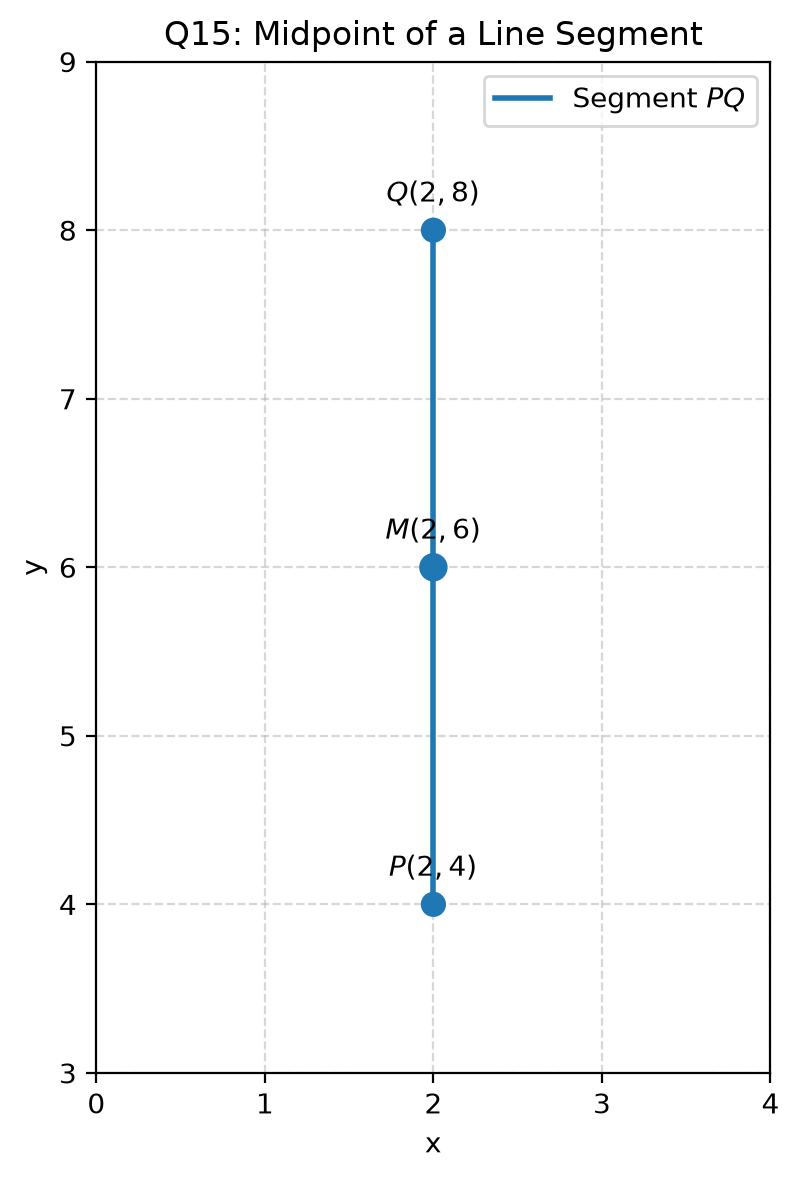
\includegraphics[width=0.45\linewidth]{figs/q15.png}
	\caption{Segment $PQ$ and its mid-point $M$}
	\label{fig:CBSE25S2-q15}
\end{figure}

\item
The area of a sector of a circle of radius $36$ cm is $54\pi$ cm$^2$. The length of the corresponding arc of the sector is
\hfill (CBSE 2025 Set 2, Q.16)
\begin{enumerate}
    \begin{multicols}{4}
        \item $8\pi\text{ cm}$
        \item $6\pi\text{ cm}$
        \item $4\pi\text{ cm}$
        \item $3\pi\text{ cm}$
    \end{multicols}
\end{enumerate}

\solution
For a sector of radius $r$ and arc length $L$,
\begin{align}
	A = \frac{1}{2}rL \implies L = \frac{2A}{r} = \frac{2\brak{54\pi}}{36} = 3\pi \text{ cm} \quad \brak{\text{Option D}}
\end{align}
The central angle is $\theta = \frac{L}{r} = \frac{\pi}{12} = 15^\circ$. The following code verifies the solution
\begin{lstlisting}[frame=single, basicstyle=\rmfamily, escapeinside={(*@}{@*)}]
(*@\makebox[\dimexpr\linewidth-2\fboxsep-2\fboxrule\relax][c]{codes/16.c}@*)
\end{lstlisting}
The following code generates \figref{fig:CBSE25S2-q16}.
\begin{lstlisting}[frame=single, basicstyle=\rmfamily, escapeinside={(*@}{@*)}]
(*@\makebox[\dimexpr\linewidth-2\fboxsep-2\fboxrule\relax][c]{codes/16plot.py}@*)
\end{lstlisting}

\item
 $\angle M = \angle B = 130^\circ$ and $\angle N = 28^\circ$. If $LM = 45$ cm, $MN = 63$ cm, $LN = 72$ cm and $AB = 5$ cm, then $AC$ is equal to
\hfill (CBSE 2025 Set 2, Q.17)
\begin{enumerate}
    \begin{multicols}{4}
        \item $16\text{ cm}$
        \item $7\text{ cm}$
        \item $8\text{ cm}$
        \item $4\text{ cm}$
    \end{multicols}
\end{enumerate}
\begin{figure}[H]
	\centering
\begin{tikzpicture}[scale=0.9, >=Stealth]
    % Triangle ABC (not to scale)
    \coordinate (A) at (0,0);
    \coordinate (B) at (2.0,1.1);
    \coordinate (C) at (3.6,0);
    \draw[thick] (A) -- (B) -- (C) -- cycle;
    \node[left] at (A) {$A$};
    \node[above] at (B) {$B$};
    \node[right] at (C) {$C$};
    \node at (2.0,0.55) {\scriptsize $130^\circ$};
    \node[above left] at (0.9,0.55) {\small $5$ cm};
    % Triangle LMN (not to scale)
    \coordinate (L) at (6,0);
    \coordinate (M) at (9.2,2.0);
    \coordinate (N) at (12.4,0);
    \draw[thick] (L) -- (M) -- (N) -- cycle;
    \node[left] at (L) {$L$};
    \node[above] at (M) {$M$};
    \node[right] at (N) {$N$};
    \node at (9.2,1.3) {\scriptsize $130^\circ$};
    \node at (11.25,0.27) {\scriptsize $28^\circ$};
    \node[above left] at (7.6,1.0) {\small $45$};
    \node[above right] at (10.8,1.0) {\small $63$};
    \node[below] at (9.2,0) {\small $72$};
\end{tikzpicture}

	\caption{Triangles $ABC$ and $LMN$ (not to scale)}
	\label{fig:CBSE25S2-q17}
\end{figure}

\solution
In $\triangle LMN$, $\angle L = 180^\circ - 130^\circ - 28^\circ = 22^\circ = \angle A$. Since $\angle A = \angle L$ and $\angle B = \angle M$, by AA similarity
\begin{align}
	\triangle LMN \sim \triangle ABC \quad \brak{L \leftrightarrow A,\ M \leftrightarrow B,\ N \leftrightarrow C}
\end{align}
The scale factor is $k = \frac{AB}{LM} = \frac{5}{45} = \frac{1}{9}$, so
\begin{align}
	AC = k \cdot LN = \frac{72}{9} = 8 \text{ cm} \quad \brak{\text{Option C}}
\end{align}
The following code verifies the solution
\begin{lstlisting}[frame=single, basicstyle=\rmfamily, escapeinside={(*@}{@*)}]
(*@\makebox[\dimexpr\linewidth-2\fboxsep-2\fboxrule\relax][c]{codes/17.c}@*)
\end{lstlisting}

\item
$\triangle DEF$ and $\triangle PQR$ are such that $\angle D = \angle Q$ and $\angle E = \angle R$. Which of the following proportions is \underline{not} true?
\hfill (CBSE 2025 Set 2, Q.18)
\begin{enumerate}
	\begin{multicols}{4}
    \item $\frac{DE}{QR} = \frac{DF}{PQ}$
    \item $\frac{EF}{RP} = \frac{DF}{PQ}$
    \item $\frac{EF}{RP} = \frac{DE}{QR}$
    \item $\frac{DE}{PQ} = \frac{EF}{RP}$
	\end{multicols}
\end{enumerate}

\solution
By AA similarity, $\triangle DEF \sim \triangle QRP$ with $D \leftrightarrow Q$, $E \leftrightarrow R$, $F \leftrightarrow P$. Corresponding sides are proportional:
\begin{align}
	\frac{DE}{QR} = \frac{EF}{RP} = \frac{DF}{QP}
\end{align}
Options A, B and C compare corresponding sides. Option D compares $DE$ with $PQ$, which are not corresponding sides. Hence the proportion that is not true is Option D. The following code checks all four options on a pair of similar triangles
\begin{lstlisting}[frame=single, basicstyle=\rmfamily, escapeinside={(*@}{@*)}]
(*@\makebox[\dimexpr\linewidth-2\fboxsep-2\fboxrule\relax][c]{codes/18.c}@*)
\end{lstlisting}

\item
If $\alpha$ and $\beta$ are the zeroes of the polynomial $x^2 - 2x - 1$, find the value of $\frac{1}{2\alpha} + \frac{1}{2\beta} + 3\alpha\beta$.
\hfill (CBSE 2025 Set 2, Q.21(b))

\solution
Let $f\brak{x} = x^2 - 2x - 1$, so $f^{\prime}\brak{x} = 2x - 2$. The Newton--Raphson iteration is
\begin{align}
	x_{n+1} = x_n - \frac{x_n^2 - 2x_n - 1}{2x_n - 2}
\end{align}
Starting from $x_0 = 2.5$ and $x_0 = -0.5$ gives
\begin{align}
	\alpha = 1 + \sqrt{2}, \quad \beta = 1 - \sqrt{2}
\end{align}
From the sum and product of zeroes, $\alpha + \beta = 2$ and $\alpha\beta = -1$, so
\begin{align}
	\frac{1}{2\alpha} + \frac{1}{2\beta} + 3\alpha\beta = \frac{\alpha+\beta}{2\alpha\beta} + 3\alpha\beta = \frac{2}{-2} - 3 = -4
\end{align}
The following code verifies the solution
\begin{lstlisting}[frame=single, basicstyle=\rmfamily, escapeinside={(*@}{@*)}]
(*@\makebox[\dimexpr\linewidth-2\fboxsep-2\fboxrule\relax][c]{codes/21b.c}@*)
\end{lstlisting}

\item
Find the smallest number which is divisible by both $644$ and $462$.
\hfill (CBSE 2025 Set 2, Q.23(a))

\solution
The required number is $\text{lcm}\brak{644,462}$. Using $644 = 2^2\cdot 7\cdot 23$ and $462 = 2\cdot 3\cdot 7\cdot 11$,
\begin{align}
	\gcd\brak{644,462} = 14, \quad
	\text{lcm}\brak{644,462} = \frac{644 \times 462}{14} = 21252
\end{align}
The following code verifies the solution (both parts of Q.23)
\begin{lstlisting}[frame=single, basicstyle=\rmfamily, escapeinside={(*@}{@*)}]
(*@\makebox[\dimexpr\linewidth-2\fboxsep-2\fboxrule\relax][c]{codes/23.c}@*)
\end{lstlisting}

\item
Two numbers are in the ratio $4:5$ and their HCF is $11$. Find their LCM.
\hfill (CBSE 2025 Set 2, Q.23(b))

\solution
Let the numbers be $4k$ and $5k$. Since $\gcd\brak{4,5} = 1$, the HCF is $k$, so $k = 11$ and the numbers are $44$ and $55$. Then
\begin{align}
	\text{lcm}\brak{44,55} = \frac{44 \times 55}{11} = 220
\end{align}
This is verified by the code for Q.23(a) above.

\item
In a school, $65\%$ of the students have black eyes, $25\%$ have brown eyes and the rest have blue eyes. A student is chosen at random. Find the probability that the student has (a) blue eyes, (b) brown or black eyes.
\hfill (CBSE 2025 Set 2, Q.27)

\solution
The probability of blue eyes is $1 - 0.65 - 0.25 = 0.10$. Order the outcomes as (Black, Brown, Blue) with probabilities $\vec{p} = \myvec{0.65 & 0.25 & 0.10}^{\top}$, and map each event to $0$ or $1$:
\begin{table}[H]
	\centering
	\begin{tabular}{|c|c|c|c|}
		\hline
		Event & Black & Brown & Blue \\ \hline
		(a) Blue & 0 & 0 & 1 \\ \hline
		(b) Brown or black & 1 & 1 & 0 \\ \hline
	\end{tabular}
	\caption{Mapping of eye colours to events}
	\label{tab:CBSE25S2-q27}
\end{table}
For an event with mapping $\vec{m}$,
\begin{align}
	\pr{E} = \vec{m}^{\top}\vec{p} \implies \text{(a) } 0.10, \quad \text{(b) } 0.65 + 0.25 = 0.90
\end{align}
The following code verifies the solution
\begin{lstlisting}[frame=single, basicstyle=\rmfamily, escapeinside={(*@}{@*)}]
(*@\makebox[\dimexpr\linewidth-2\fboxsep-2\fboxrule\relax][c]{codes/27.c}@*)
\end{lstlisting}

\item
In the figure, $PC$ is a tangent to the circle at $C$ and $AB$ is a diameter which, when extended, meets the tangent at $P$. If $\angle PCA = 110^\circ$, find $\angle CBA$ and $\angle BCO$.
\hfill (CBSE 2025 Set 2, Q.29)
\begin{figure}[H]
	\centering
\begin{tikzpicture}[scale=1.3, >=Stealth]
    \coordinate (O) at (0,0);
    \coordinate (A) at (-2,0);
    \coordinate (B) at (2,0);
    \coordinate (C) at (1.5321,1.2856);
    \coordinate (P) at (2.6108,0);
    \draw[thick] (O) circle (2);
    \draw[thick] (A) -- (P);
    \draw[thick] (P) -- (C);
    \draw[thick] (A) -- (C) -- (B);
    \draw[thick] (O) -- (C);
    \fill (O) circle (1.3pt) (A) circle (1.3pt) (B) circle (1.3pt)
          (C) circle (1.3pt) (P) circle (1.3pt);
    \node[below] at (O) {$O$};
    \node[left] at (A) {$A$};
    \node[below] at (B) {$B$};
    \node[above] at (C) {$C$};
    \node[below right] at (P) {$P$};
    \draw (C)++(-160:0.4) arc[start angle=-160, end angle=-50, radius=0.4];
    \node[fill=white, inner sep=0.5pt] at (1.30,0.62) {\scriptsize $110^\circ$};
\end{tikzpicture}

	\caption{Tangent $PC$ and diameter $AB$}
	\label{fig:CBSE25S2-q29}
\end{figure}

\solution
Since $AB$ is a diameter, $\angle ACB = 90^\circ$. As $P$ lies beyond $B$,
\begin{align}
	\angle PCA = \angle PCB + \angle BCA \implies \angle PCB = 110^\circ - 90^\circ = 20^\circ
\end{align}
By the tangent--chord theorem, $\angle CAB = \angle PCB = 20^\circ$. In $\triangle ABC$,
\begin{align}
	\angle CBA = 90^\circ - 20^\circ = 70^\circ
\end{align}
Since $OB = OC$, $\triangle OBC$ is isosceles and
\begin{align}
	\angle BCO = \angle CBO = 70^\circ
\end{align}
The following code verifies the solution
\begin{lstlisting}[frame=single, basicstyle=\rmfamily, escapeinside={(*@}{@*)}]
(*@\makebox[\dimexpr\linewidth-2\fboxsep-2\fboxrule\relax][c]{codes/29.c}@*)
\end{lstlisting}

\item
Find the coordinates of the points which divide the line segment joining $A\brak{-2,2}$ and $B\brak{2,8}$ into four equal parts.
\hfill (CBSE 2025 Set 2, Q.31(b))

\solution
With $\vec{A} = \myvec{-2\\2}$ and $\vec{B} = \myvec{2\\8}$, $\vec{B}-\vec{A} = \myvec{4\\6}$. The division points are $\vec{A} + \frac{k}{4}\brak{\vec{B}-\vec{A}}$ for $k = 1,2,3$:
\begin{align}
	\vec{P} = \myvec{-1 \\ 3.5}, \quad \vec{Q} = \myvec{0 \\ 5}, \quad \vec{R} = \myvec{1 \\ 6.5}
\end{align}
The following code verifies the solution
\begin{lstlisting}[frame=single, basicstyle=\rmfamily, escapeinside={(*@}{@*)}]
(*@\makebox[\dimexpr\linewidth-2\fboxsep-2\fboxrule\relax][c]{codes/31b.c}@*)
\end{lstlisting}
The following code generates \figref{fig:CBSE25S2-q31b}.
\begin{lstlisting}[frame=single, basicstyle=\rmfamily, escapeinside={(*@}{@*)}]
(*@\makebox[\dimexpr\linewidth-2\fboxsep-2\fboxrule\relax][c]{codes/31bplot.py}@*)
\end{lstlisting}
\begin{figure}[H]
	\centering
	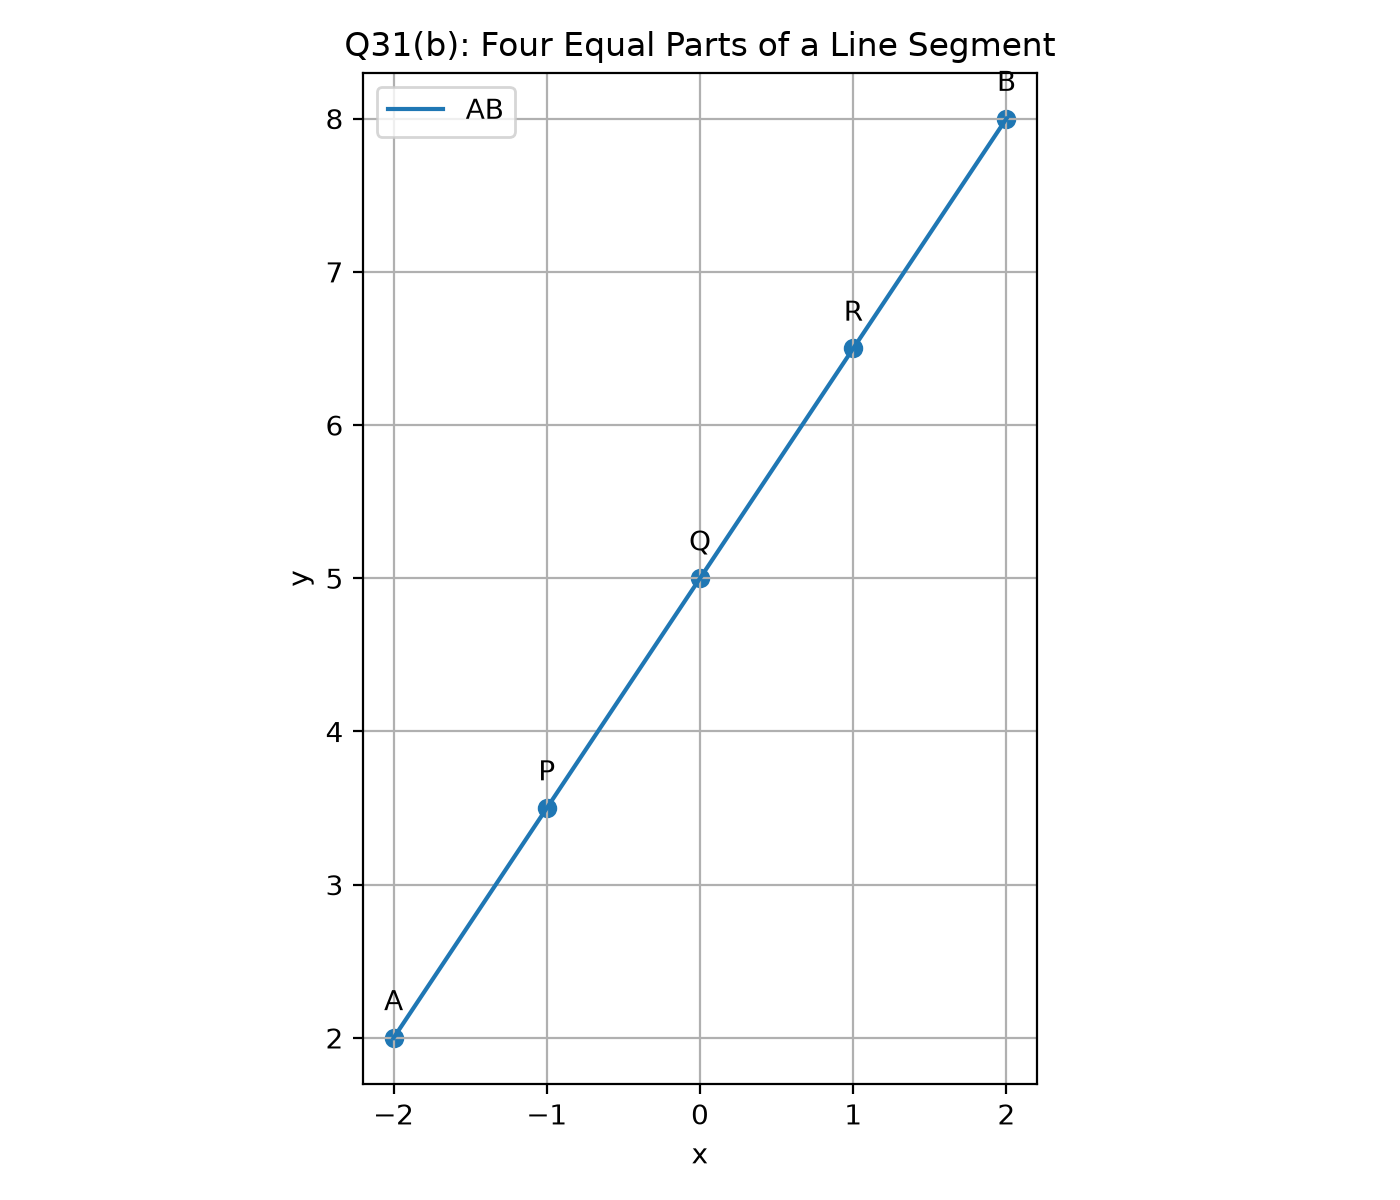
\includegraphics[width=0.5\linewidth]{figs/q31b.png}
	\caption{Division of $AB$ into four equal parts}
	\label{fig:CBSE25S2-q31b}
\end{figure}

\item
The $n^{\text{th}}$ term of an AP is $4$, its common difference is $2$ and the sum of its first $n$ terms is $-14$. Find $n$, the first term, and the sum of the first $20$ terms.
\hfill (CBSE 2025 Set 2, Q.32(a))

\solution
Let the first term be $a$. Then $a_n = a + \brak{n-1}d = 4$ gives $a = 6 - 2n$. Using $S_n = \frac{n}{2}\brak{a + a_n}$,
\begin{align}
	-14 = \frac{n}{2}\brak{6 - 2n + 4} = n\brak{5 - n}
	\implies n^2 - 5n - 14 = 0 \implies \brak{n-7}\brak{n+2} = 0
\end{align}
Since $n > 0$, $n = 7$ and $a = 6 - 14 = -8$. Then
\begin{align}
	S_{20} = \frac{20}{2}\sbrak{2\brak{-8} + 19\brak{2}} = 220
\end{align}
The following code verifies the solution
\begin{lstlisting}[frame=single, basicstyle=\rmfamily, escapeinside={(*@}{@*)}]
(*@\makebox[\dimexpr\linewidth-2\fboxsep-2\fboxrule\relax][c]{codes/32a.c}@*)
\end{lstlisting}

\item
A vessel in the form of an inverted cone of height $8$ cm and radius $5$ cm is filled with water to the brim. Lead shots, each a sphere of radius $0.5$ cm, are dropped into the vessel until one-fourth of the water flows out. Find the number of lead shots dropped.
\hfill (CBSE 2025 Set 2, Q.33)

\solution
The volume of water in the cone is
\begin{align}
	V_c = \frac{1}{3}\pi R^2 h = \frac{1}{3}\pi\brak{5}^2\brak{8} = \frac{200\pi}{3} \text{ cm}^3
\end{align}
The water that flows out equals the total volume of the shots, so the volume displaced is $\frac{V_c}{4} = \frac{50\pi}{3}$ cm$^3$. Each shot has volume
\begin{align}
	V_s = \frac{4}{3}\pi r^3 = \frac{4}{3}\pi\brak{0.5}^3 = \frac{\pi}{6} \text{ cm}^3
\end{align}
Therefore the number of shots is
\begin{align}
	N = \frac{50\pi/3}{\pi/6} = 100
\end{align}
The following code verifies the solution
\begin{lstlisting}[frame=single, basicstyle=\rmfamily, escapeinside={(*@}{@*)}]
(*@\makebox[\dimexpr\linewidth-2\fboxsep-2\fboxrule\relax][c]{codes/33.c}@*)
\end{lstlisting}

\item
A man lent part of his money at $10\%$ per annum and the rest at $15\%$ per annum. His yearly interest was \rupee 1900. Had he interchanged the two rates, he would have earned \rupee 200 more. Find the two amounts.
\hfill (CBSE 2025 Set 2, Q.34)

\solution
Let $x$ and $y$ be the amounts lent at $10\%$ and $15\%$. Then
\begin{align}
	0.10x + 0.15y &= 1900 \\
	0.15x + 0.10y &= 2100
\end{align}
In matrix form,
\begin{align}
	\myvec{0.10 & 0.15 \\ 0.15 & 0.10}\myvec{x \\ y} = \myvec{1900 \\ 2100}
\end{align}
The determinant is $0.10^2 - 0.15^2 = -0.0125$, and by Cramer's rule
\begin{align}
	x = \frac{1900\brak{0.10} - 0.15\brak{2100}}{-0.0125} = 10000, \quad
	y = \frac{0.10\brak{2100} - 0.15\brak{1900}}{-0.0125} = 6000
\end{align}
Hence the amounts are \rupee 10000 at $10\%$ and \rupee 6000 at $15\%$. The following code verifies the solution
\begin{lstlisting}[frame=single, basicstyle=\rmfamily, escapeinside={(*@}{@*)}]
(*@\makebox[\dimexpr\linewidth-2\fboxsep-2\fboxrule\relax][c]{codes/34.c}@*)
\end{lstlisting}

\item
\textbf{Case study (rainfall).} The distribution of the number of meteorological subdivisions by annual rainfall is given below.
\hfill (CBSE 2025 Set 2, Q.36)
\begin{table}[H]
	\centering
	\begin{tabular}{|c|c|c|c|c|c|c|}
		\hline
		Rainfall (mm) & 200--400 & 400--600 & 600--800 & 800--1000 & 1000--1200 & 1200--1400 \\ \hline
		Subdivisions & 3 & 4 & 7 & 4 & 3 & 3 \\ \hline
	\end{tabular}
	\caption{Rainfall distribution, total $24$ subdivisions}
	\label{tab:CBSE25S2-q36}
\end{table}
(i) Find the modal class. (ii) Find the median rainfall \textbf{or} the mean rainfall. (iii) Find the number of subdivisions with rainfall of at least $800$ mm.

\solution
\textbf{(i)} The highest frequency is $7$, so the modal class is $600$--$800$ mm.

\textbf{(ii)} Here $N = 24$ and $\frac{N}{2} = 12$. The cumulative frequencies are $3, 7, 14, 18, 21, 24$, so the median class is $600$--$800$ with $l = 600$, $cf = 7$, $f = 7$, $h = 200$:
\begin{align}
	\text{Median} = l + \frac{\frac{N}{2} - cf}{f}\times h = 600 + \frac{12-7}{7}\times 200 \approx 742.86 \text{ mm}
\end{align}
For the mean, with class marks $x_i = 300, 500, \dots, 1300$,
\begin{align}
	\bar{x} = \frac{\sum f_i x_i}{\sum f_i} = \frac{18600}{24} = 775 \text{ mm}
\end{align}
\textbf{(iii)} The classes from $800$ mm upward have $4 + 3 + 3 = 10$ subdivisions.

The following code verifies the solution
\begin{lstlisting}[frame=single, basicstyle=\rmfamily, escapeinside={(*@}{@*)}]
(*@\makebox[\dimexpr\linewidth-2\fboxsep-2\fboxrule\relax][c]{codes/36.c}@*)
\end{lstlisting}

\item
\textbf{Case study (lighthouse).} A lighthouse $AB$ is $50$ m high. From its top $B$, the angles of depression of a ship at $P$ and, after some time, at $Q$ are $30^\circ$ and $45^\circ$ respectively, with $P$, $Q$, $A$ on the same line.
\hfill (CBSE 2025 Set 2, Q.38)
% TODO: part (ii) of the paper is not included - its exact wording was not verified
\begin{figure}[H]
	\centering
\begin{tikzpicture}[scale=1.2, >=Stealth]
    \coordinate (A) at (0,0);
    \coordinate (B) at (0,2.5);
    \coordinate (Q) at (2.5,0);
    \coordinate (P) at (4.3301,0);
    \draw[thick] (-0.6,0) -- (5.0,0);
    \draw[ultra thick] (A) -- (B);
    \draw[thick] (B) -- (Q);
    \draw[thick] (B) -- (P);
    \draw[dashed] (B) -- (5.0,2.5);
    \fill (A) circle (1.5pt) (B) circle (1.5pt) (Q) circle (1.5pt) (P) circle (1.5pt);
    \node[below left] at (A) {$A$};
    \node[above left] at (B) {$B$};
    \node[below] at (Q) {$Q$};
    \node[below] at (P) {$P$};
    \node[left] at (0,1.25) {\small $50$ m};
    \draw (B)++(1.0,0) arc[start angle=0, end angle=-45, radius=1.0];
    \draw (B)++(2.0,0) arc[start angle=0, end angle=-30, radius=2.0];
    \node[fill=white, inner sep=0.5pt] at (1.62,2.18) {\scriptsize $45^\circ$};
    \node[fill=white, inner sep=0.5pt] at (2.55,2.18) {\scriptsize $30^\circ$};
\end{tikzpicture}

	\caption{Lighthouse $AB$ and ship positions $P$, $Q$}
	\label{fig:CBSE25S2-q38}
\end{figure}

\solution
\textbf{(i)} In $\triangle QAB$, $\tan 45^\circ = \frac{AB}{QA}$, so
\begin{align}
	QA = \frac{50}{\tan 45^\circ} = 50 \text{ m}
\end{align}
\textbf{(iii)(a)} In $\triangle PAB$, $\tan 30^\circ = \frac{AB}{PA}$, so $PA = 50\sqrt{3}$ m, and the distance moved from $P$ to $Q$ is
\begin{align}
	PQ = PA - QA = 50\brak{\sqrt{3} - 1} \approx 36.60 \text{ m}
\end{align}
\textbf{(iii)(b)} The ship covers $QA = 50$ m $= 0.05$ km in $10$ minutes $= \frac{1}{6}$ h, so
\begin{align}
	\text{Speed} = \frac{0.05}{1/6} = 0.3 \text{ km/h}
\end{align}
The following code verifies the solution
\begin{lstlisting}[frame=single, basicstyle=\rmfamily, escapeinside={(*@}{@*)}]
(*@\makebox[\dimexpr\linewidth-2\fboxsep-2\fboxrule\relax][c]{codes/38.c}@*)
\end{lstlisting}

\end{enumerate}
